% vim: ai sw=2 spell spelllang=cs

\section{Parsery}
\frame{\sectionpage}

\begin{frame}
  \frametitle{Parsery}

  \begin{itemize}
    \item Analyzátor jazyka
    \begin{itemize}
      \item Přirozeného, \emph{programovacího}, \dots
    \end{itemize}

    \pause

    \item Výstupem je nějaký lépe zpracovatelný popis jazyka
    \begin{itemize}
      \item Např.\ informace v grafu nebo stromu
      \item Několik mezifází, jak toho dosáhnout
      \item Projdeme si na dalších slidech
    \end{itemize}

    \pause

    \item Získané informace se dále využijí
    \begin{itemize}
      \item K překladu do jiného jazyka (např.\ strojového)
      \item K interpretaci
      \item \dots
    \end{itemize}

    \pause

    \item Detailněji o jazycích a parserech např.\ v ,,Dragon Book''
  \end{itemize}

\end{frame}

\begin{frame}
  \frametitle{Výroba parseru}

  \begin{enumerate}

    \item Ručně psané
    \begin{itemize}
      \item Rychlost parseru a explicita
      \item \textsc{gcc} (\heading{Demo})
    \end{itemize}

    \pause
    \medskip

    \item Generované nástroji
    \begin{itemize}
      \item Rychlost napsání parseru a přehlednost kódu
      \item \textsc{Lex}+\textsc{Yacc}
      \item \textsc{Flex}+\textsc{Bison}
      \item \emph{\ant}
      \item A další
    \end{itemize}

  \end{enumerate}

\end{frame}

\begin{frame}
  \frametitle{\ant}

  \begin{itemize}
  \item Nástroj ke generování parserů
  \item Psaný v Javě
  \item Vstup je LL(\textasteriskcentered) gramatika (shora-dolů, čitelná)

  \item Generuje parsery do různých jazyků
  \begin{itemize}
    \item Java, C, C\texttt{++}, C\#, \dots
    \item Podpora pro C jen ve verzi 3 (pro 4 se připravuje)
  \end{itemize}

  \end{itemize}

\end{frame}

\begin{frame}
  \frametitle{Úkol}

  \heading{Stáhněte a zprovozněte si \ant 3}
  \begin{enumerate}
    \item \url{http://www.antlr3.org/download.html}
    \begin{itemize}
      \item Ukládejte do \file{pb173-bin/02/}
      \item \textsc{AntlrWorks}: ,,Version 1.5''
      \item \ant: ,,Complete \ant 3.5.2 Java binaries jar''
    \end{itemize}

    \item Knihovna pro C (\file{libantlr3c} a \file{antlr3c-devel})
    \begin{itemize}
      \item RPM: \href{http://software.opensuse.org/package/libantlr3c2}{\nolinkurl{http://software.opensuse.org}}
      \item Zdroje: \url{http://www.antlr3.org/download/C/}
    \end{itemize}

    \item Vyzkoušejte generovat \file{Parser.g} z \file{pb173-bin/02/test/}
    \begin{itemize}
      \item \cmd{make}
      \item Spousty varování ignorujte
    \end{itemize}

    \item Pusťte jej
    \begin{itemize}
      \item \cmd{./parser test_input}
      \item Změňte \file{test_input} a zkuste znovu
    \end{itemize}

  \end{enumerate}

\end{frame}

\begin{frame}[fragile]
  \frametitle{Části parseru}

  \begin{center}
  \tikzstyle{pre} = [<-,shorten <=1pt,>=stealth',semithick]
  \begin{tikzpicture}[node distance=5mm, font=\footnotesize]
      \node [tl_state] (S) {Zdroj};
      \node [tl_phase] (LEX) [right=of S, align=center] {Lexikální \\ analýza}
	edge [pre] node {} (S);
      \node [tl_state] (TOK) [right=of LEX] {Tokeny}
	edge [pre] node {} (LEX);
      \node [tl_phase] (PAR) [right=of TOK, align=center] {Syntaktická \\ analýza}
	edge [pre] node {} (TOK);
      \node [tl_state] (AST) [right=of PAR] {AST}
	edge [pre] node {} (PAR);
      \node [tl_state] (CFG) [above right=of AST] {CFG}
	edge [pre,dashed] node {} (AST);
      \node [tl_state] (OTH) [below right=of AST] {\dots}
	edge [pre,dashed] node {} (AST);
  \end{tikzpicture}
\end{center}


  \begin{enumerate}
    \item Lexikální analýza
    \begin{itemize}
      \item Převod sekvence znaků na sekvenci ,,tokenů''
      \begin{itemize}
	\item Např.\ ,,\code{int a}'' převede na ,,\code{KEYWORD:int ID:a}''
      \end{itemize}
    \end{itemize}

    \pause

    \item Syntaktická analýza
    \begin{itemize}
      \item Dává sekvence tokenů smysl?
      \item Ano $\Rightarrow$ sémantická analýza

      \begin{itemize}
	\item Přímá interpretace, tvorba AST, \dots
      \end{itemize}
    \end{itemize}

  \end{enumerate}

\end{frame}

\begin{frame}[fragile]
  \frametitle{Vnitřní struktury parseru}

  \begin{center}
  \begin{tabular}{ccc}
    \begin{lstlisting}[columns=fullflexible]
  void fun(int a)
  { /* comment */
    int b = 0;
    if (a)
      b = 5;
    a = 3 * b;
  }
    \end{lstlisting} & $\Rightarrow$ &
    \begin{lstlisting}[columns=fullflexible]
key:void id:fun LPAR key:int id:a RPAR
LCUR
  key:int id:b EQ num:0 SEMIC
  key:if LPAR id:a RPAR
    id:b EQ num:5 SEMIC
  id:a EQ num:3 MULT id:b SEMIC
RCUR
    \end{lstlisting}
  \end{tabular}
  \end{center}

  \pause

  \begin{center}
    \tikzset{ast/.style={thick,draw,minimum size=5mm}}
    \tikzset{ast_hl/.style={ast, bottom color=black!10, top color=black!10}}
    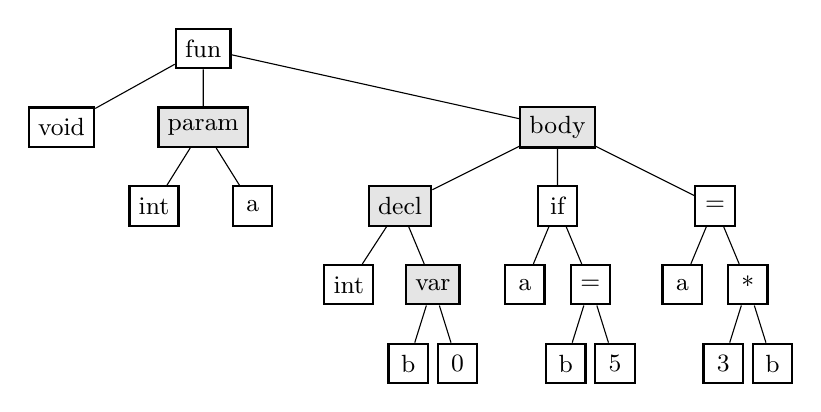
\begin{tikzpicture}[level/.style={sibling distance = 2.5cm/#1,
    level distance = 1cm}, font=\small]
      \node [ast] {\code{fun}}
	  child [sibling distance=1.8cm] { node [ast] {\code{void}} }
	  child { node [ast_hl] {param}
	    child { node [ast] {\code{int}} }
	    child { node [ast] {\code{a}} }
	  }
	  child [sibling distance=4.5cm] { node [ast_hl] {body}
	    child [sibling distance=2cm] { node [ast_hl] {decl}
	      child [sibling distance=1.3cm] { node [ast] {\code{int}} }
	      child { node [ast_hl] (L_1) {var}
		child { node [ast] {\code{b}} }
		child { node [ast] {\code{0}} }
	      }
	    }
	    child [sibling distance=2cm] { node [ast] {\code{if}}
	      child { node [ast] (L_2) {\code{a}} }
	      child { node [ast] (L_3) {\code{=}}
		child { node [ast] {\code{b}} }
		child { node [ast] {\code{5}} }
	      }
	    }
	    child [sibling distance=2cm] { node [ast] (L_4) {\code{=}}
	      child { node [ast] {\code{a}} }
	      child { node [ast] {\code{*}}
		child { node [ast] {\code{3}} }
		child { node [ast] {\code{b}} }
	      }
	    }
	  }
	  ;
    \end{tikzpicture}
  \end{center}

\end{frame}

\begin{frame}[fragile]{Formát \ant}

  \heading{Formát celého souboru pro \ant}
  \begin{lstlisting}[language=XML, columns=fullflexible]
grammar Jmeno; // shoda s nazvem souboru
options {
  language = C; // vystupni jazyk parseru
}
@header {
#define X	10
  // vlozi se na zacatek generovaneho parseru
}
@members {
  static void moje_funkce() { ... }
  // vlozi se za hlavicku parseru
}

pravidlo1
  : pravidlo2
  | pravidlo3;
...
  \end{lstlisting}

\end{frame}

\begin{frame}[fragile]
  \frametitle{Části parseru v \ant}

  \heading{\ant obsahuje obě části v jednom souboru}
  \begin{itemize}
    \item 2 typy pravidel
    \begin{itemize}
      \item Počáteční \emph{velké} písmeno -- lexikální
      \item Počáteční \emph{malé} písmeno -- syntaktická
    \end{itemize}

    \pause

    \item \code{;} odděluje pravidla

    \pause

    \item \code{:} odděluje levou a pravou stranu pravidla
  \end{itemize}

  \onslide<1->

  \begin{block}{Příklad}
  \begin{lstlisting}[language=XML, columns=fullflexible]
/* syntakticka analyza */
helloWorld
  : AHOJ SVETE
  | SVETE AHOJ { puts("Nepise se to obracene?"); }
  ;

/* lexikalni analyza */
AHOJ : 'Ahoj' ;
SVETE : 'Svete' ;
  \end{lstlisting}
  \end{block}

\end{frame}

\begin{frame}
  \frametitle{Pravá strana pravidel}

  \begin{itemize}
    \item \code{|} odděluje možnosti
    \begin{itemize}
      \item Více možností: \code{zvirata : savci | obojzivelnici ;}
      \item Také kombinace podčástí: \code{strunatci : ('pe'|'ko') 's' ;}
    \end{itemize}

    \pause

    \item Opakování pravidla
    \begin{itemize}
      \item \code{pravidlo?} -- 0--1krát, např.\ \code{nicNeboX : 'x'? ;}
      \item \code{pravidlo*} -- 0--$\infty$krát, např.\ \code{kolonaAut : 'auto'* ;}
      \item \code{pravidlo+} -- 1--$\infty$krát, např.\ \code{zvukHada : 's'+ ;}
    \end{itemize}

    \pause

    \item Rozsahy
    \begin{itemize}
      \item \code{'A'..'Z'} -- celá velká ASCII abeceda
    \end{itemize}

    \pause

    \item Speciální pravidlo pro konec souboru: \code{EOF}
    \begin{itemize}
      \item Donutí číst celý soubor
    \end{itemize}
  \end{itemize}

\end{frame}

\begin{frame}[fragile]
  \frametitle{Úkol}

  \heading{Rozšíření gramatiky}
  \begin{enumerate}
    \item Prozkoumejte obsah \file{02/test/Parser.g}
    \item Vytvořte si token \code{NUMBER} pro čísla
    \begin{itemize}
      \item \code{('0'..'9')+}
    \end{itemize}

    \item Vytvořte si tokeny pro \code{\+} a \code{\-}
    \item Vytvořte si nové pravidlo \code{expr} pro tyto 2 operace
    \begin{itemize}
      \item Bude obsahovat 2 možnosti (oddělené \code{|})
      \item Pro sčítání např.\ \code{NUMBER PLUS NUMBER}
    \end{itemize}

    \item Přidejte do \code{translationUnit} novou možnost
    \begin{itemize}
      \item Bude odpovídat 1--$\infty$ opakováním \code{expr}
    \end{itemize}

    \item Vyzkoušejte nově podporované vstupy
    \begin{itemize}
      \item \code{1+2}, \code{100-10}, apod.
    \end{itemize}
  \end{enumerate}

\end{frame}

\mysection{Akce pravidel}

\begin{frame}[fragile]
  \frametitle{Akce pravidel}

  \heading{Pravidla mohou obsahovat akce}
  \begin{itemize}
    \item Kód spouštěný při určitých událostech
    \item \code{\{ C code \}} za pravostrannými tokeny
    \item Vykoná se ihned, když token odpovídá vstupu
  \end{itemize}

  \begin{block}{Příklad}
  \begin{lstlisting}[language=XML, columns=fullflexible]
p : ID {
    puts("found an ID");
  } ID {
    puts("found second ID");
  } ID {
    puts("wow, 3 IDs");
  }
  ;
  \end{lstlisting}
  \end{block}

\end{frame}

\begin{frame}
  \frametitle{Úkol}

  \heading{Akce pravidel}
  \begin{enumerate}
    \item Dopište akce na konec obou možností \code{expr}
    \item Vypište nějaký text
    \begin{itemize}
      \item Ale různý pro každou možnost
    \end{itemize}
    \item Vyzkoušejte
  \end{enumerate}

\end{frame}

\begin{frame}[fragile]
  \frametitle{Vlastnosti tokenů}

  \heading{Každý token má vlastnosti}
  \begin{itemize}
    \item \code{line} -- zdrojový řádek
    \item \code{pos} -- zdrojový sloupec

    \pause

    \item \code{text} -- tokenizovaný řetězec (,,Ahoj'' pro AHOJ)
    \begin{itemize}
      \item Jak pro tokeny (pravé strany), tak pro pravidla (levé strany)
      \item Typ: \code{pANTLR3_STRING}, obsahuje \code{char *chars}
    \end{itemize}

    \pause

    \item Akce můžou odkazovat předcházející tokeny
    \begin{itemize}
      \item Implicitně jménem tokenu/pravidla: \code{p : NUMBER \{ \$NUMBER.line; \} ;}

      \pause

      \item Nebo pojmenováním: \code{p : n1=NUMBER PLUS n2=NUMBER \{ \$n2.pos; \} ;}
    \end{itemize}

  \end{itemize}

  \onslide<1->

  \begin{block}{Příklad}
  \begin{lstlisting}[language=XML, columns=fullflexible,belowskip=0pt]
helloWorld : x=AHOJ y=SVETE {
      printf("line=\%d col=\%d\n", $x.line, $x.pos);
  \end{lstlisting}
  \onslide<2->
  \begin{lstlisting}[language=XML, columns=fullflexible,aboveskip=0pt,belowskip=0pt]
      printf("x=\%s y=\%s whole=\%s\n", $x.text->chars, $y.text->chars, $helloWorld.text->chars);
  \end{lstlisting} %stopzone
  \onslide<1->
  \begin{lstlisting}[language=XML, columns=fullflexible,aboveskip=0pt]
  } ;
  \end{lstlisting}
  \end{block}

\end{frame}

\begin{frame}
  \frametitle{Úkol}

  \heading{Vlastnosti pravidel}
  \begin{enumerate}
    \item Pro každou operaci sčítání/odčítání
    \begin{itemize}
      \item Vypište číslo řádku a sloupce pro obě čísla (\code{\$NUMBER.line} a
	\code{\$NUMBER.pos})
      \item Vypište obě čísla jako řetězec (\code{\$NUMBER.text->chars})
    \end{itemize}
    \item Vyzkoušejte roztroušením textu po testovacím vstupu
  \end{enumerate}

\end{frame}

\begin{frame}[fragile]
  \frametitle{Předávání hodnot}

  \heading{Každé pravidlo muže akceptovat/vracet hodnotu}
  \begin{itemize}
    \item Stejně jako funkce
    \item \code{levaStrana[type1 param1, ...] returns [typeR ret] : pravaStrana;}
    \begin{itemize}
      \item Pak lze v akcích odkazovat na \code{\$param1} typu \code{type1}
      \item Akce \emph{musí} nastavovat \code{\$ret} typu \code{typeR}
    \end{itemize}
  \end{itemize}

  \begin{block}{Příklad}
  \begin{lstlisting}[language=XML, columns=fullflexible]
translationUnit
        : expr[5] EOF { printf("I'm done \%d\n", $expr.ret); }
;

expr[int par] returns [int ret]
  : n1=NUMBER PLUS n2=NUMBER {
    $ret = $par * atoi($n1.text->chars) + atoi($n2.text->chars);
  }
  | SVETE AHOJ { $ret = 0; }
  ;
  \end{lstlisting} %stopzone
  \end{block}

\end{frame}

\begin{frame}
  \frametitle{Úkol}

  \heading{Vlastnosti pravidel}
  \begin{enumerate}
    \item Vytvořte si pravidlo pro čísla
    \begin{itemize}
      \item \code{number : NUMBER ;}
    \end{itemize}

    \item Z něj a z \code{expr} si vracejte (smysluplnou) hodnotu
    \begin{itemize}
      \item Tj.\ počítejte
    \end{itemize}

    \item V \code{translationUnit} vypište výsledek
    \begin{itemize}
      \item Pro každé \code{expr}
    \end{itemize}
  \end{enumerate}

\end{frame}

\begin{frame}[fragile]
  \frametitle{Inicializace/ukončení}

  \heading{Každé pravidlo muže mít inicializace/ukončení}
  \begin{itemize}
    \item Na konci levé strany pravidla (před dvojtečkou)
    \item Před aplikováním pravidla: \code{@init\{ ... \}}
    \begin{itemize}
      \item Např.\ inicializovat proměnné
    \end{itemize}
    \item Po aplikování pravidla: \code{@after\{ ... \}}
    \begin{itemize}
      \item Např.\ počítání
    \end{itemize}
  \end{itemize}

  \begin{block}{Příklad}
  \begin{lstlisting}[language=XML, columns=fullflexible]
expr[int par] returns [int ret]
@init{ $ret = 0; }
@after{ $ret--; }
  : n1=NUMBER PLUS n2=NUMBER {
    $ret = $par * atoi($n1.text->chars) + atoi($n2.text->chars);
  }
  ;
  \end{lstlisting} %stopzone
  \end{block}

\end{frame}

%\begin{frame}[fragile]
%  \frametitle{Tvorba AST}
%
%  \begin{itemize}
%    \item Do \code{options}
%    \begin{itemize}
%      \item \code{ASTLabelType = pANTLR3_BASE_TREE;}
%      \item \code{output = AST;}
%    \end{itemize}
%
%    \item Kořenem je uzel tvořený počátečním symbolem gramatiky
%    \item Podstromy se připojují ve vnořených pravidlech
%    \begin{itemize}
%      \item Pomocí speciálních přepisovacích pravidel
%      \item Explicitně: \code{pravaStrana -> podstromAST}
%      \begin{itemize}
%	\item \code{^(KOREN pravaStrana)}
%	\item \code{KOREN} musí být v token nebo v \code{tokens}
%      \end{itemize}
%
%      \item Implicitně: \code{pravaStrana} (vytvoří podstrom \code{pravaStrana})
%      \begin{itemize}
%	\item \code{^} -- kořen (pod)stromu
%	\item \code{!} -- nevkládat do stromu
%      \end{itemize}
%    \end{itemize}
%  \end{itemize}
%
%  \begin{lstlisting}[language=XML, columns=fullflexible]
%statement
%  : expression^ ';'! // implicitni strom
%  | e1=expression '+' e2=expression ';' -> ^(BINARY_OP '+' e1 e2)
%  \end{lstlisting}
%
%\end{frame}
%
%\begin{frame}
%  \frametitle{Úkol}
%
%  \heading{Dopište tvorbu stromu do gramatiky \file{test/Parser.g}}
%  \begin{enumerate}
%    \item Nejprve přesuňte \file{test/Parser.g} do \file{parser/Parser.g}
%    \begin{itemize}
%    \item Je zde již podpora pro AST
%    \end{itemize}
%
%    \item Definujte token \code{KOREN}
%    \begin{itemize}
%    \item V sekci \code{tokens}
%    \end{itemize}
%
%    \item Explicitně vytvořte AST podstromy v \code{helloWorld}
%    \begin{itemize}
%      \item Např.\ \code{AHOJ} \code{SVETE} přepište na
%        \code{^(KOREN AHOJ SVETE)}
%    \end{itemize}
%  \end{enumerate}
%
%\end{frame}
%
%\begin{frame}
%  \frametitle{Co s AST?}
%
%  \begin{itemize}
%    \item Vypsat (viz \file{main.c})
%    \begin{itemize}
%      \item \code{puts((char *)parseTree.tree-> toStringTree(parseTree.tree)->chars);}
%    \end{itemize}
%
%    \pause
%
%    \item Vytvořit novou stromovou gramatiku
%      \begin{itemize}
%	\item Čte AST
%	\item Nemusí se starat o původní jazyk
%	\item Provádí akce na podstromech
%	\begin{itemize}
%	  \item Interpretuje je
%	  \item Překládá
%	  \item Vytváří graf toku řízení
%	  \item \dots
%	\end{itemize}
%
%	\pause
%
%	\item \code{tree grammar JmenoAST;} v hlavičce
%	\item \code{tokenVocab = JmenoGramatiky;} v \code{options}
%
%	\pause
%
%	\item Pravidla podle generovaných: \code{^(BINARY_OP '+' e1 e2)}
%	\item Na pravé straně může být akce: \\
%	\code{\{ printf("\\\%s + \\\%s\\n", \$e1.text->chars, \$e2.text->chars);\ \}}
%      \end{itemize}
%  \end{itemize}
%
%\end{frame}
%
%\begin{frame}
%  \frametitle{Úkol}
%
%  \heading{Napište stromovou gramatiku pro \file{Parser.g}}
%  \begin{enumerate}
%    \item Vytvořte nový soubor ASTParser.g (nebo použijte ukázkový)
%
%    \item Zapište všechny možné AST stromy, které generujete v \file{Parser.g}
%    \begin{itemize}
%      \item Můžete strukturovat za použití pravidel a rekurze
%    \end{itemize}
%
%    \item A vypište si ke každému pravidlu jeho jednotlivé části
%    \begin{itemize}
%      \item \code{p : X \{ puts(\$X.text->chars); \} ;}
%    \end{itemize}
%  \end{enumerate}
%
%\end{frame}
